\documentclass[a4paper]{article}

\usepackage[paper=a4paper, left=1.5cm, right=1.5cm, bottom=1.5cm, top=3.5cm]{geometry}
\usepackage[spanish,activeacute]{babel}
\usepackage[latin1]{inputenc}
\usepackage{amsthm}
\usepackage{amsmath}
\usepackage{amsfonts}
\usepackage{amssymb}
\usepackage{alltt}
\usepackage{graphicx} %Para incluir el logo de la UBA
\usepackage{caratula} %Para armar el cuadro de integrantes
\usepackage{multirow} %Para poder poner varias lineas juntas sin divisiones en una tabla
\usepackage[lined,ruled,linesnumbered]{algorithm2e}
\usepackage{algpseudocode}
\usepackage{scrextend}
\usepackage{blindtext}


%Cosas para escribir codigo fuente
%Fuente: http://en.wikibooks.org/wiki/LaTeX/Source_Code_Listings
\usepackage{listings}
\usepackage{color}

\setcounter{secnumdepth}{5}

\definecolor{mygreen}{rgb}{0,0.6,0}
\definecolor{mygray}{rgb}{0.5,0.5,0.5}
\definecolor{myorange}{rgb}{1,0.4,0.2}
\definecolor{myblue}{rgb}{0,0,0.65}

%Configuracion para los listings
\lstset{ %
  backgroundcolor=\color{white},   % choose the background color; you must add \usepackage{color} or \usepackage{xcolor}
  basicstyle=\small,        % the size of the fonts that are used for the code
  breakatwhitespace=false,         % sets if automatic breaks should only happen at whitespace
  breaklines=true,                 % sets automatic line breaking
  captionpos=b,                    % sets the caption-position to bottom
  commentstyle=\color{mygreen},    % comment style
  deletekeywords={...},            % if you want to delete keywords from the given language
  escapeinside={\%*}{*)},          % if you want to add LaTeX within your code
  extendedchars=true,              % lets you use non-ASCII characters; for 8-bits encodings only, does not work with UTF-8
  frame=single,                    % adds a frame around the code
  keywordstyle=\color{myblue},       % keyword style
  language=Octave,                 % the language of the code
  morekeywords={*,...},            % if you want to add more keywords to the set
  numbers=left,                    % where to put the line-numbers; possible values are (none, left, right)
  numbersep=5pt,                   % how far the line-numbers are from the code
  numberstyle=\tiny\color{mygray}, % the style that is used for the line-numbers
  rulecolor=\color{black},         % if not set, the frame-color may be changed on line-breaks within not-black text (e.g. comments (green here))
  showspaces=false,                % show spaces everywhere adding particular underscores; it overrides 'showstringspaces'
  showstringspaces=false,          % underline spaces within strings only
  showtabs=false,                  % show tabs within strings adding particular underscores
  stepnumber=1,                    % the step between two line-numbers. If it's 1, each line will be numbered
  stringstyle=\color{myorange},     % string literal style
  tabsize=2,                       % sets default tabsize to 2 spaces
  title=\lstname                   % show the filename of files included with \lstinputlisting; also try caption instead of title
}

\renewcommand{\lstlistingname}{C\'{o}digo}

\lstset{language=C++,caption={Descriptive Caption Text},label=DescriptiveLabel}

\setlength\parindent{0pt}
%\topmargin = -1cm
%\textheight = 24cm 

\begin{document}

\integrante{Sclar, Melanie}{551/12}{melaniesclar@gmail.com}
\integrante{Zylber, Ariel}{530/12}{arielzylber@gmail.com}
\integrante{Hardy, Gonzalo}{449/09}{hardy.gonzalo@gmail.com}
\integrante{Fixman, Mart\'in}{391/11}{martinfixman@gmail.com}
\integrante{Aleman, Dami\'an Eliel}{377/10}{damianealeman@gmail.com}

\def\Materia{Ingenier\'ia del Software 1}
\def\Titulo{Trabajo Pr\'actico 2}
\def\Fecha{19 de Octubre de 2014}

%----- CARATULA -----%

\thispagestyle{empty}

\begin{center}
	
\includegraphics[scale = 0.25]{logo_uba.jpg}
\end{center}

\vspace{5mm}

\begin{center}
	{\textbf{\large UNIVERSIDAD DE BUENOS AIRES}}\\[1.5em]
	{\textbf{\large Departamento de Computaci\'{o}n}}\\[1.5em]
    {\textbf{\large Facultad de Ciencias Exactas y Naturales}}\\
    \vspace{35mm}
    {\LARGE\textbf{\Materia}}\\[1em]    
    \vspace{15mm}
    {\Large \textbf{\Titulo}}\\[1em]
    \vspace{15mm}
    {\textbf{\Large \Fecha}}\\
    \vspace{15mm}
    \textbf{\tablaints}
\end{center}

\newtheorem{teo}{Teorema}[section]
\newtheorem{propo}{Proposici\'{o}n}[section]
\newtheorem{lema}{Lema}[section]
\newtheorem{coro}{Corolario}[section]
\newtheorem{defi}{Definici\'{o}n}[section]

\newpage
\thispagestyle{empty}
\tableofcontents

\parskip=5pt
\setlength{\parindent}{0pt}

\newpage
\setcounter{page}{1}
\pagenumbering{arabic}
\pagestyle{plain}

\newpage


\newcommand{\Asig}{\ensuremath{\leftarrow}}
\newcommand{\AndY}{\ensuremath{\wedge}}
\newcommand{\Or}{\ensuremath{\vee}}
\newcommand{\Not}{\ensuremath{\neg}}
\newcommand{\NotEq}{\ensuremath{\neq}}
\newcommand{\MayorIg}{\ensuremath{\geq}}
\newcommand{\tabu}{\hspace*{0.7cm}}
\newcommand{\ctabu}{\hspace*{0.8cm}}
\newcommand{\htabu}{\hspace*{0.35cm}}
\newcommand{\moduloNombre}[1]{\textbf{#1}}



\section{Diagrama de Casos de Uso}

A continuaci\'on exponemos el diagrama de casos de uso bas\'andonos en el primer tp presentado:
\\
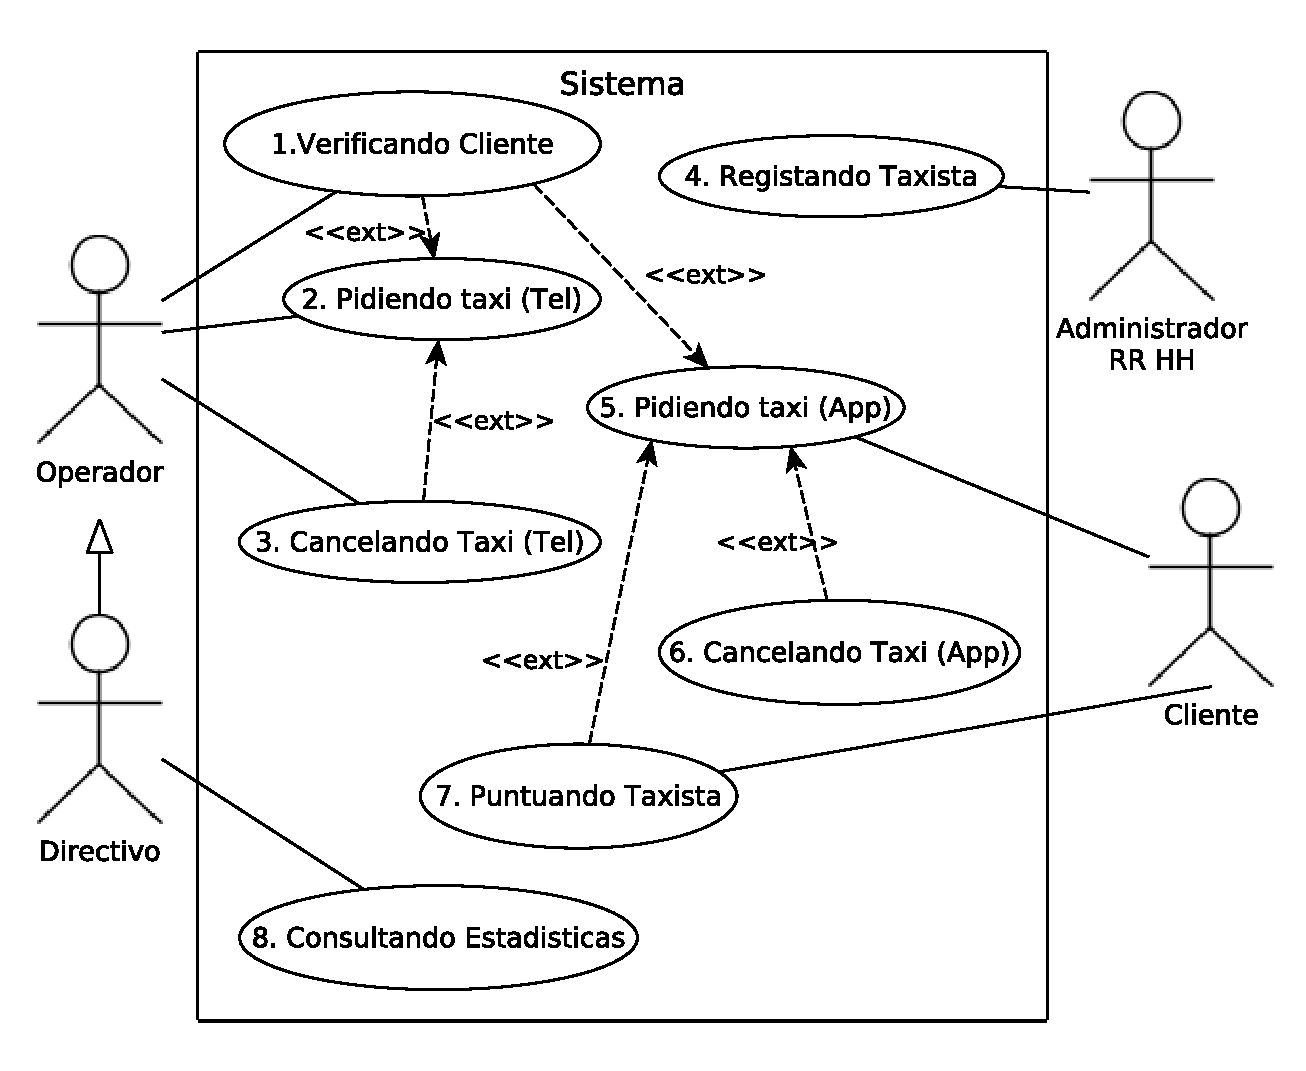
\includegraphics[scale=0.38]{diag_CasosDeUso.pdf}

En los lugares donde hubiere un O-ref en el diagrama de objetivos, decidimos tomar la alternativa m\'as fiel al enunciado original: optamos por no utilizar una remiser\'ia para los viajes regulares, y por no implementar la alternativa de los mensajes de texto.
\section{Casos de Uso}


\subsection{Caso de Uso \textit{Verificando Cliente (Tel\'efono)}}
\begin{center}
\begin{tabular}{|p{10cm} | p{6cm}|}
\hline
\multicolumn{2}{|p{16cm}|}{\textbf{Descripci\'on:} Se verifica si el cliente est\'a registrado. Si no lo est\'a, se le pide los datos y se lo registra en el sistema.} \\
\hline
\multicolumn{2}{|l|}{\textbf{Actor:} Operador} \\
\hline
\multicolumn{2}{|l|}{\textbf{Pre:} -} \\
\hline
\multicolumn{2}{|p{14cm}|}{\textbf{Post:} Se verifica que el usuario est\'a registrado, y si no lo estaba se lo registra en el sistema.}\\
\hline
\textbf{Curso Normal}  & \textbf{Curso Alternativo} \\ \hline
1. El sistema solicita el nombre completo del usuario. & \\ \hline
2. El operador ingresa el nombre completo. & \\ \hline
3. El sistema busca los datos del usuario. Si no los encuentra, EXTIENDE CASO DE USO \textit{Registrando Cliente}. & \\ \hline
4. Fin caso de uso & \\ \hline
\end{tabular}
\end{center}

\subsection{Caso de Uso \textit{Registrando Cliente (Tel\'efono)}}
\begin{center}
\begin{tabular}{|p{10cm} | p{6cm}|}
\hline
\multicolumn{2}{|p{16cm}|}{\textbf{Descripci\'on:} Se registra al nuevo cliente en el sistema.} \\
\hline
\multicolumn{2}{|l|}{\textbf{Actor:} Operador} \\
\hline
\multicolumn{2}{|l|}{\textbf{Pre:} El cliente a registrar no est\'a a\'un en el sistema.} \\
\hline
\multicolumn{2}{|p{14cm}|}{\textbf{Post:} El nuevo cliente est\'a registrado en el sistema.}\\
\hline
\textbf{Curso Normal}  & \textbf{Curso Alternativo} \\ \hline
1. El sistema solicita los datos del nuevo cliente. & \\ \hline
2. El operador ingresa todos los datos personales del cliente. & \\ \hline
3. El sistema informa que el nuevo cliente fue registrado en el sistema. & 3.1 Si el sistema no pudo agregar al nuevo cliente, se informa este hecho y se va al paso 1. \\ \hline
4. Fin caso de uso & \\ \hline
\end{tabular}
\end{center}

\subsection{Caso de Uso \textit{Pidiendo Taxi (Tel\'efono)}}
\begin{center}
\begin{tabular}{|p{10cm} | p{6cm}|}
\hline
\multicolumn{2}{|p{15cm}|}{\textbf{Descripci\'on:} El cliente pide un taxi telef\'onicamente.} \\
\hline
\multicolumn{2}{|p{15cm}|}{\textbf{Actor:} Operador } \\
\hline
\multicolumn{2}{|p{15cm}|}{\textbf{Pre:} El cliente desea pedir un viaje y lo har\'a telef\'onicamente.} \\
\hline
\multicolumn{2}{|p{15cm}|}{\textbf{Post:} Un taxi se env\'ia seg\'un el pedido del cliente. Una vez que el taxi comienza a moverse, se muestra su posici\'on a trav\'es de la aplicaci\'on. }\\
\hline
\textbf{Curso Normal}  & \textbf{Curso Alternativo} \\ \hline
1. El operador recibe una llamada de un cliente que desea pedir un taxi y USA CASO DE USO \textit{Verificando Cliente}. Adem\'as le anuncia al sistema que se desea pedir un nuevo viaje. & \\ \hline
2. El sistema solicita saber si el viaje es simple o regular, y en este \'ultimo caso, cada cu\'anto se realizar\'a el viaje. & \\ \hline
3. El operador ve e informa sobre las posibles opciones de viaje, y una vez elegido el tipo de viaje deseado env\'ia los datos sobre el tipo de viaje y su periodicidad. & \\ \hline
4. El sistema env\'ia una copia de los datos seleccionados y pide una confirmaci\'on de los mismos. & \\ \hline
5. El operador confirma que los datos del viaje son correctos (tanto del horario como la regularidad del mismo). & 5.1. Si los datos son incorrectos, ir al paso 2. \\ \hline
6. El sistema carga el dato de nuevo viaje, y elige un taxi autom\'aticamente y USA CASO DE USO \textit{Confirmando viaje}. & 6.1. Si el taxista rechaza el viaje, volver a paso 6. \\ \hline
7. Fin de caso de uso. & \\ \hline
\end{tabular}
\end{center}

\subsection{Caso de Uso \textit{Confirmando viaje}}
\begin{center}
\begin{tabular}{|p{8cm} | p{8cm}|}
\hline
\multicolumn{2}{|p{16cm}|}{\textbf{Descripci\'on:} Se env\'ia una solicitud de nuevo pedido a la terminal m\'ovil del taxi elegido. Se confirma la aceptaci\'on del pedido, y se comienza a dirigir hacia la direcci\'on desde donde se pidi\'o el taxi. } \\
\hline
\multicolumn{2}{|p{15cm}|}{\textbf{Actor:} Terminal m\'ovil} \\
\hline
\multicolumn{2}{|p{15cm}|}{\textbf{Pre:} Se sabe a qu\'e taxi se le pedir\'a que realice el viaje. Tambi\'en se sabe la direcci\'on desde donde se pidi\'o el viaje.} \\
\hline
\multicolumn{2}{|p{15cm}|}{\textbf{Post:} La terminal m\'ovil inform\'o que se acept\'o el pedido y se comenzar\'a }\\
\hline
\textbf{Curso Normal}  & \textbf{Curso Alternativo} \\ \hline
1. El sistema le env\'ia un pedido para realizar un nuevo viaje a la terminal m\'ovil (inform\'andole la direcci\'on del mismo). & \\ \hline %%% SI NO SE PUEDE COMUNICAR CON LA TERMINAL?
2. La terminal m\'ovil muestra este nuevo pedido y espera a que se lo acepte (al aceptarlo, se compromete a comenzar a dirigirse a la direcci\'on indicada). Luego se avisa la aceptaci\'on al sistema. & 2.1. Si se rechaza el pedido, la terminal se lo informa al sistema. \newline 2.2. Si pasan m\'as de 3 minutos con la terminal m\'ovil mostrando el nuevo pedido y no se lo responde, se asume que fue rechazado y se act\'ua igual que si se hubiera rechazado activamente. \\ \hline
3. Fin de caso de uso. & \\ \hline
\end{tabular}
\end{center}

\subsection{Caso de Uso \textit{Cancelando Taxi (Tel\'efono)}}
\begin{center}
\begin{tabular}{|p{10cm} | p{6cm}|}
\hline
\multicolumn{2}{|p{15cm}|}{\textbf{Descripci\'on:} Se cancela el pedido de un viaje pedido telef\'onicamente.} \\
\hline
\multicolumn{2}{|p{15cm}|}{\textbf{Actor:} Operador, Terminal m\'ovil} \\
\hline
\multicolumn{2}{|p{15cm}|}{\textbf{Pre:} El viaje que se desea cancelar ya fue pedido pero todav\'ia no fue realizado. El viaje fue pedido telef\'onicamente. El operador ya conoce qu\'e viaje se desea cancelar.} \\
\hline
\multicolumn{2}{|p{15cm}|}{\textbf{Post:} El viaje es cancelado, informando al taxista de su cancelaci\'on y borr\'andolo de los viajes a realizar.}\\
\hline
\textbf{Curso Normal}  & \textbf{Curso Alternativo} \\ \hline
1. El operador recibe un pedido de un cliente para cancelar cierto viaje, e ingresa el nombre del cliente que desea cancelar el viaje. & \\ \hline
2. El sistema muestra todos los viajes pedidos por el cliente que a\'un no fueron realizados (simples y regulares). & 2.1. Si el cliente no figura como registrado en el sistema, el sistema informa que no se encuentra registrado (y asimismo, el operador se lo informar\'a al cliente). \\ \hline
3. El operador selecciona el viaje a cancelar seg\'un los dichos del cliente. Si se quiere cancelar el pedido regular de un taxi (no se quiere recibir m\'as el servicio de ese viaje regular), EXTIENDE CASO DE USO \textit{Cancelar viaje regular (Tel\'efono)}. \newline Si se quiere cancelar un \'unico viaje, EXTIENDE CASO DE USO \textit{Cancelar viaje simple (Tel\'efono)}. & 3.1. Si no existen viajes pendientes, el sistema informa la imposibilidad de cancelar un viaje. \\ \hline %% ACA HAY UN TEMITA CON EL SIGUIENTE CASO: SI ES JUEVES Y TE LLAMO PARA DECIRTE "MIRA, MAÑANA VIERNES POR FAVOR NO ME MANDES EL TAXI PERO SEGUI MANDANDOMELO TODOS LOS VIERNES" QUE ONDA.
%Para mi que cancele los viajes regulares y a la semana que viene que lo pida de vuelta...
4. Fin de caso de uso. & \\ \hline
\end{tabular}
\end{center}

\subsection{Caso de Uso \textit{Cancelando Viaje Simple (Tel\'efono)}}
\begin{center}
\begin{tabular}{|p{10cm} | p{6cm}|}
\hline
\multicolumn{2}{|p{16cm}|}{\textbf{Descripci\'on:} Se cancela un \'unico viaje, pedido telef\'onicamente. } \\
\hline
\multicolumn{2}{|l|}{\textbf{Actor:} Operador, Terminal m\'ovil} \\
\hline
\multicolumn{2}{|l|}{\textbf{Pre:} Ya se seleccion\'o un viaje para cancelar.} \\
\hline
\multicolumn{2}{|p{16cm}|}{\textbf{Post:} El viaje fue cancelado y al taxi dirigi\'endose al domicilio se le inform\'o de esta cancelaci\'on.}\\
\hline
\textbf{Curso Normal}  & \textbf{Curso Alternativo} \\ \hline
1. El operador informa que se quiere cancelar un cierto viaje, y el mismo es simple. & \\ \hline
2. El sistema da de baja el pedido de su listado de viajes a realizar, y USA CASO DE USO \textit{Cancelando movilizaci\'on de taxi}. El sistema informa que el pedido fue cancelado exitosamente. & \\ \hline
3. El operador informa al cliente que ya fue cancelado su pedido. & \\ \hline
4. Fin de caso de uso. & \\ \hline
\end{tabular}
\end{center}

\subsection{Caso de Uso \textit{Cancelando Viaje Regular (Tel\'efono)}}
\begin{center}
\begin{tabular}{|p{10cm} | p{6cm}|}
\hline
\multicolumn{2}{|p{16cm}|}{\textbf{Descripci\'on:} Se cancela un viaje regular, pedido telef\'onicamente. } \\
\hline
\multicolumn{2}{|l|}{\textbf{Actor:} Operador, Terminal m\'ovil} \\
\hline
\multicolumn{2}{|l|}{\textbf{Pre:} Ya se seleccion\'o un viaje para cancelar, y es regular. } \\
\hline
\multicolumn{2}{|p{16cm}|}{\textbf{Post:} El viaje regular fue cancelado (ya no se recibir\'a m\'as el servicio), y si hab\'ia un taxi dirigi\'endose al domicilio, se cancel\'o este env\'io.}\\
\hline
\textbf{Curso Normal}  & \textbf{Curso Alternativo} \\ \hline
1. El operador informa que se quiere cancelar un cierto viaje, y el mismo es regular. & \\ \hline
2. El sistema da de baja el pedido de su listado de viajes a realizar, y si ya hab\'ia sido enviado un taxi al domicilio, EXTIENDE CASO DE USO \textit{Cancelando movilizaci\'on de taxi}. El sistema informa que el pedido fue cancelado exitosamente. & \\ \hline
3. El operador informa al cliente que ya fue cancelado su pedido. & \\ \hline
4. Fin de caso de uso. & \\ \hline
\end{tabular}
\end{center}

\subsection{Caso de Uso \textit{Registrando taxista}}
\begin{center}
\begin{tabular}{|p{10cm} | p{6cm}|}
\hline
\multicolumn{2}{|p{15cm}|}{\textbf{Descripci\'on:} Se registra a un nuevo taxista en la lista de taxistas de la empresa del sistema.} \\
\hline
\multicolumn{2}{|l|}{\textbf{Actor:} Administrador RRHH } \\
\hline
\multicolumn{2}{|p{15cm}|}{\textbf{Pre:} Se seleccion\'o un taxista para contratar, y el taxista seleccionado todav\'ia no es parte de la empresa. } \\
\hline
\multicolumn{2}{|p{15cm}|}{\textbf{Post:} Se agreg\'o al nuevo taxista a la flota de la empresa (la lista de taxistas de la empresa en el sistema). }\\
\hline
\textbf{Curso Normal}  & \textbf{Curso Alternativo} \\ \hline
1. El administrador solicita agregar a un nuevo taxista al sistema. & \\ \hline
2. El sistema pide los datos del nuevo taxista a agregar. & \\ \hline
3. El administrador ingresa los datos del nuevo taxista. & \\ \hline
4. El sistema informa que se agreg\'o correctamente al taxista a la flota. Se pide precisar en qu\'e taxi se encontrar\'a dicho taxista. & 4.1 Si el taxista ya era parte de la flota, el sistema informa que es imposible agregarlo y retorna al paso 2. \\ \hline
5. El administrador ingresa en qu\'e taxi de la empresa se encontrar\'a el nuevo taxista. & \\ \hline
6. El sistema informa que se agreg\'o correctamente el taxi del nuevo taxista & Si no se pudo agregar, volver al paso 4. \\ \hline
7. Fin de caso de uso. & \\ \hline

\end{tabular}
\end{center}

\subsection{Caso de Uso \textit{Verificando Cliente (Aplicaci\'on)}}
\begin{center}
\begin{tabular}{|p{10cm} | p{6cm}|}
\hline
\multicolumn{2}{|p{16cm}|}{\textbf{Descripci\'on:} Se verifica si el cliente est\'a registrado. Si no lo est\'a, se le pide los datos y se lo registra en el sistema.} \\
\hline
\multicolumn{2}{|l|}{\textbf{Actor:} Aplicaci\'on para celular} \\
\hline
\multicolumn{2}{|l|}{\textbf{Pre:} -} \\
\hline
\multicolumn{2}{|p{14cm}|}{\textbf{Post:} Se verifica que el usuario est\'a registrado, y si no lo estaba se lo registra en el sistema.}\\
\hline
\textbf{Curso Normal}  & \textbf{Curso Alternativo} \\ \hline
1. El sistema solicita el nombre completo del usuario. & \\ \hline
2. La aplicaci\'on muestra la solicitud e ingresa el nombre completo. & \\ \hline
3. El sistema busca los datos del usuario. Si no los encuentra, EXTIENDE CASO DE USO \textit{Registrando Cliente}. & \\ \hline
4. Fin caso de uso & \\ \hline
\end{tabular}
\end{center}

\subsection{Caso de Uso \textit{Registrando Cliente (Aplicaci\'on)}}
\begin{center}
\begin{tabular}{|p{10cm} | p{6cm}|}
\hline
\multicolumn{2}{|p{16cm}|}{\textbf{Descripci\'on:} Se registra al nuevo cliente en el sistema.} \\
\hline
\multicolumn{2}{|l|}{\textbf{Actor:} Aplicaci\'on para celular} \\
\hline
\multicolumn{2}{|l|}{\textbf{Pre:} El cliente a registrar no est\'a a\'un en el sistema.} \\
\hline
\multicolumn{2}{|p{14cm}|}{\textbf{Post:} El nuevo cliente est\'a registrado en el sistema.}\\
\hline
\textbf{Curso Normal}  & \textbf{Curso Alternativo} \\ \hline
1. El sistema solicita los datos del nuevo cliente. & \\ \hline
2. La aplicaci\'on muestra la solicitud e ingresa todos los datos personales del cliente. & \\ \hline
3. El sistema informa que el nuevo cliente fue registrado en el sistema. & 3.1 Si el sistema no pudo agregar al nuevo cliente, se informa este hecho y se va al paso 1. \\ \hline
4. Fin caso de uso & \\ \hline
\end{tabular}
\end{center}


\subsection{Caso de Uso \textit{Pidiendo Taxi (Aplicaci\'on)}}
\begin{center}
\begin{tabular}{|p{10cm} | p{6cm}|}
\hline
\multicolumn{2}{|p{15cm}|}{\textbf{Descripci\'on:} El cliente pide un taxi v\'ia la aplicaci\'on de acuerdo con sus preferencias. } \\
\hline
\multicolumn{2}{|p{15cm}|}{\textbf{Actor:} Aplicaci\'on para celulares } \\
\hline
\multicolumn{2}{|p{15cm}|}{\textbf{Pre:} El cliente desea pedir un viaje y lo har\'a via la aplicaci\'on. El cliente se encuentra verificado. } \\
\hline
\multicolumn{2}{|p{15cm}|}{\textbf{Post:} Un taxi se env\'ia seg\'un el pedido del cliente. Una vez que el taxi comienza a moverse, se muestra su posici\'on a trav\'es de la aplicaci\'on. }\\
\hline
\textbf{Curso Normal}  & \textbf{Curso Alternativo} \\ \hline
1. La aplicaci\'on le anuncia al sistema que se desea pedir un nuevo viaje. & \\ \hline
2. El sistema solicita saber si el viaje es simple o regular, y en este \'ultimo caso, cada cu\'anto se realizar\'a el viaje. & \\ \hline
3. La aplicaci\'on informa sobre las posibles opciones de viaje, y una vez elegido el tipo de viaje deseado env\'ia los datos sobre el tipo de viaje y su periodicidad. & \\ \hline
4. El sistema carga estos datos, y si se trata de un viaje simple, EXTIENDE CASO DE USO \textit{Eligiendo Taxi}. Si se trata de un viaje regular, EXTIENDE CASO DE USO \textit{Eligiendo perfil de taxi}. & \\ \hline
5. El sistema env\'ia una copia de los datos seleccionados y pide una confirmaci\'on de los mismos. & \\ \hline
6. La aplicaci\'on confirma que los datos son correctos (tanto del taxi como del horario y la regularidad del mismo). & 6.1 Si los datos son incorrectos, ir al paso 2. \\ \hline
7. Si el viaje es simple, el usuario ya eligi\'o un taxi. Si el viaje es regular, el sistema elige el mejor taxi de acuerdo a las preferencias del cliente. Luego, no importa si el viaje es regular o simple, USA CASO DE USO \textit{Confirmando viaje}. & 6.1. Si el taxista rechaza el viaje y era un viaje simple, la aplicaci\'on lo informa adecuadamente y se vuelve al paso 4. Si era un viaje regular, volver al paso 7. \\ \hline
8. La aplicaci\'on informa que el taxi ya fue enviado a destino y USA CASO DE USO \textit{Enviando ubicaci\'on del taxi} para informar la ubicaci\'on del taxi. & \\ \hline
9. Fin de caso de uso. & \\ \hline
\end{tabular}
\end{center}

\subsection{Caso de Uso \textit{Eligiendo taxi}}
\begin{center}
\begin{tabular}{|p{10cm} | p{6cm}|}
\hline
\multicolumn{2}{|p{16cm}|}{\textbf{Descripci\'on:} El usuario, a trav\'es de la aplicaci\'on, elige qu\'e taxi desea en base a sus preferencias.} \\
\hline
\multicolumn{2}{|p{15cm}|}{\textbf{Actor:} Aplicaci\'on para celular} \\
\hline
\multicolumn{2}{|p{15cm}|}{\textbf{Pre:} El usuario que utiliza la aplicaci\'on est\'a verificado. Se est\'a pidiendo un viaje simple v\'ia la aplicaci\'on.} \\
\hline
\multicolumn{2}{|p{15cm}|}{\textbf{Post:} Se seleccion\'o un taxi para enviar a destino.}\\
\hline
\textbf{Curso Normal}  & \textbf{Curso Alternativo} \\ \hline
1. El sistema brinda informaci\'on sobre taxis y taxistas disponibles.  & \\ \hline
2. La aplicaci\'on muestra la informaci\'on sobre taxis y taxistas disponibles. & \\ \hline
3. A trav\'es de la aplicaci\'on se selecciona el taxi deseado, y \'esta se lo informa al sistema. & \\ \hline
4. El sistema guarda la selecci\'on del taxi. & \\ \hline
5. Fin de caso de uso. & \\ \hline
\end{tabular}
\end{center}

\subsection{Caso de Uso \textit{Eligiendo perfil de taxi}}
\begin{center}
\begin{tabular}{|p{10cm} | p{6cm}|}
\hline
\multicolumn{2}{|p{16cm}|}{\textbf{Descripci\'on:} El usuario, a trav\'es de la aplicaci\'on, elige qu\'e perfil de taxi desea.} \\
\hline
\multicolumn{2}{|p{15cm}|}{\textbf{Actor:} Aplicaci\'on para celular } \\
\hline
\multicolumn{2}{|p{15cm}|}{\textbf{Pre:} El usuario que utiliza la aplicaci\'on est\'a verificado. El viaje que se est\'a pidiendo es regular, v\'ia la aplicaci\'on.} \\
\hline
\multicolumn{2}{|p{15cm}|}{\textbf{Post:} Se seleccion\'o un perfil de taxi para enviar a destino.}\\
\hline
\textbf{Curso Normal}  & \textbf{Curso Alternativo} \\ \hline
1. El sistema brinda informaci\'on sobre los perfiles que se pueden elegir (las condiciones preferidas sobre el taxi o taxista a enviar).  & \\ \hline
2. La aplicaci\'on muestra la informaci\'on sobre los perfiles disponibles. & \\ \hline
3. A trav\'es de la aplicaci\'on se selecciona el o los perfiles deseados, y \'esta se lo informa al sistema. & \\ \hline
4. El sistema guarda la selecci\'on del taxi. & \\ \hline
5. Fin de caso de uso. & \\ \hline
\end{tabular}
\end{center}


\subsection{Caso de Uso \textit{Cancelando Taxi (Aplicaci\'on)}}
\begin{center}
\begin{tabular}{|p{10cm} | p{6cm}|}
\hline
\multicolumn{2}{|p{16cm}|}{\textbf{Descripci\'on:} Se cancela el pedido de un viaje.} \\
\hline
\multicolumn{2}{|l|}{\textbf{Actor:} Aplicaci\'on para celulares, Terminal m\'ovil} \\ %%%% AGREGUE UN ACTOR
\hline
\multicolumn{2}{|p{15cm}|}{\textbf{Pre:} El viaje que se desea cancelar ya fue pedido pero todav\'ia no fue realizado. } \\
\hline
\multicolumn{2}{|p{15cm}|}{\textbf{Post:} El viaje es cancelado, informando al taxista de su cancelaci\'on y borr\'andolo de los viajes a realizar.}\\
\hline
\textbf{Curso Normal}  & \textbf{Curso Alternativo} \\ \hline
1. La aplicaci\'on solicita la cancelaci\'on de un viaje. & \\ \hline
2. El sistema env\'ia los datos de todos los viajes pedidos pero a\'un no realizados (los viajes regulares entran en esta categor\'ia). & \\ \hline
3. La aplicaci\'on muestra el listado de viajes pedidos a\'un no realizados, y se selecciona el viaje a cancelar enviando al sistema c\'ual es. & \\ \hline
4. El sistema recibe esta informaci\'on e informa la cancelaci\'on del viaje. Luego USA CASO DE USO \textit{Cancelando movilizaci\'on de taxi} & \\ \hline %%% QUE PASA SI TODAVIA NO HABIA SIDO ASIGNADO UN TAXISTA?????
5. La aplicaci\'on recibe la confirmaci\'on de cancelaci\'on y la muestra. & \\ \hline
6. Fin de caso de uso. & \\ \hline
\end{tabular}
\end{center}

\subsection{Caso de Uso \textit{Cancelando Viaje Simple (Aplicaci\'on)}}
\begin{center}
\begin{tabular}{|p{10cm} | p{6cm}|}
\hline
\multicolumn{2}{|p{16cm}|}{\textbf{Descripci\'on:} Se cancela un \'unico viaje, pedido v\'ia la aplicaci\'on. } \\
\hline
\multicolumn{2}{|l|}{\textbf{Actor:} Aplicaci\'on para celulares, Terminal m\'ovil} \\
\hline
\multicolumn{2}{|l|}{\textbf{Pre:} Ya se seleccion\'o un viaje para cancelar. El usuario est\'a verificado.} \\
\hline
\multicolumn{2}{|p{16cm}|}{\textbf{Post:} El viaje fue cancelado y al taxi dirigi\'endose al domicilio se le inform\'o de esta cancelaci\'on.}\\
\hline
\textbf{Curso Normal}  & \textbf{Curso Alternativo} \\ \hline
1. La aplicaci\'on informa que se quiere cancelar un cierto viaje, y el mismo es simple. & \\ \hline
2. El sistema da de baja el pedido de su listado de viajes a realizar, y USA CASO DE USO \textit{Cancelando movilizaci\'on de taxi}. El sistema informa que el pedido fue cancelado exitosamente. & \\ \hline
3. La aplicaci\'on informa que ya fue cancelado el pedido. & \\ \hline
4. Fin de caso de uso. & \\ \hline
\end{tabular}
\end{center}

\subsection{Caso de Uso \textit{Cancelando Viaje Regular (Aplicaci\'on)}}
\begin{center}
\begin{tabular}{|p{10cm} | p{6cm}|}
\hline
\multicolumn{2}{|p{16cm}|}{\textbf{Descripci\'on:} Se cancela un viaje regular, pedido v\'ia la aplicaci\'on. } \\
\hline
\multicolumn{2}{|l|}{\textbf{Actor:} Aplicaci\'on para celular, Terminal m\'ovil} \\
\hline
\multicolumn{2}{|l|}{\textbf{Pre:} Ya se seleccion\'o un viaje para cancelar, y es regular. El usuario est\'a verificado.} \\
\hline
\multicolumn{2}{|p{16cm}|}{\textbf{Post:} El viaje regular fue cancelado (ya no se recibir\'a m\'as el servicio), y si hab\'ia un taxi dirigi\'endose al domicilio, se cancel\'o este env\'io.}\\
\hline
\textbf{Curso Normal}  & \textbf{Curso Alternativo} \\ \hline
1. La aplicaci\'on informa que se quiere cancelar un cierto viaje, y el mismo es regular. & \\ \hline
2. El sistema da de baja el pedido de su listado de viajes a realizar, y si ya hab\'ia sido enviado un taxi al domicilio, EXTIENDE CASO DE USO \textit{Cancelando movilizaci\'on de taxi}. El sistema informa que el pedido fue cancelado exitosamente. & \\ \hline
3. La aplicaci\'on informa que ya fue cancelado el pedido. & \\ \hline
4. Fin de caso de uso. & \\ \hline
\end{tabular}
\end{center}

\subsection{Caso de Uso \textit{Cancelando movilizaci\'on de taxi}}
\begin{center}
\begin{tabular}{|p{10cm} | p{6cm}|}
\hline
\multicolumn{2}{|p{16cm}|}{\textbf{Descripci\'on:} Se informa a la terminal m\'ovil que el viaje que hab\'ia sido aceptado fue cancelado por el cliente.} \\
\hline
\multicolumn{2}{|p{15cm}|}{\textbf{Actor:} Terminal m\'ovil} \\
\hline
\multicolumn{2}{|p{15cm}|}{\textbf{Pre:} El viaje a cancelar fue asignado al taxi sobre el que se encuentra la terminal m\'ovil, y todav\'ia no fue realizado.} \\
\hline
\multicolumn{2}{|p{15cm}|}{\textbf{Post:} El viaje pedido fue cancelado.}\\
\hline
\textbf{Curso Normal}  & \textbf{Curso Alternativo} \\ \hline
1. El sistema env\'ia a la terminal m\'ovil la informaci\'on de que el viaje actual ha sido cancelado. & \\ \hline
2. La terminal m\'ovil muestra esta informaci\'on, y env\'ia una confirmaci\'on de recepci\'on una vez que el taxista lo haya le\'ido. & \\ \hline
3. El sistema recibe la confirmaci\'on de recepci\'on. & 3.1 Si luego de un tiempo determinado no se recibe la confirmaci\'on, volver a paso 1. \\  \hline
4. Fin de caso de uso. & \\ \hline
\end{tabular}
\end{center}

\subsection{Caso de Uso \textit{Puntuando Taxista}}
\begin{center}
\begin{tabular}{|p{10cm} | p{6cm}|}
\hline
\multicolumn{2}{|p{16cm}|}{\textbf{Descripci\'on:} El cliente punt\'ua al taxista seg\'un su experiencia del viaje, y su opini\'on se carga en el sistema.} \\
\hline
\multicolumn{2}{|l|}{\textbf{Actor:} Aplicaci\'on para celulares } \\
\hline
\multicolumn{2}{|p{15.5cm}|}{\textbf{Pre:} El cliente realiz\'o un viaje con el taxista puntuado y a\'un no lo evalu\'o por ese viaje (si realiz\'o m\'as de un viaje con el taxista, tiene que tener al menos un viaje por el que no lo puntu\'o). El cliente est\'a verificado y el viaje que desea puntuar fue pedido por la aplicaci\'on.} \\
\hline
\multicolumn{2}{|p{14cm}|}{\textbf{Post:} La opini\'on y el puntaje del cliente sobre el taxista es cargado en el sistema. }\\
\hline
\textbf{Curso Normal}  & \textbf{Curso Alternativo} \\ \hline
1. La aplicaci\'on informa que se solicit\'o dar una opini\'on sobre un taxista. & \\ \hline
2. El sistema carga y env\'ia la informaci\'on de todos los taxistas de viajes que a\'un no fueron puntuados. & \\ \hline
3. La aplicaci\'on recibe los datos y muestra el listado de taxistas de viajes que a\'un no fueron puntuados y luego se selecciona el taxista de qu\'e viaje desea puntuar.  & \\ \hline
4. Una vez seleccionado el taxista a puntuar, la aplicaci\'on muestra una interfaz donde puntuar y opcionalmente dejar un mensaje explicativo acerca de la satisfacci\'on con el servicio. Una vez se haya terminado se emitir la opini\'on, la misma se env\'ia al sistema. & \\ \hline
5. El sistema carga la opini\'on y el puntaje del cliente sobre el taxista del viaje seleccionado. El sistema informa que el puntaje fue cargado exitosamente. & 5.1 Si el sistema no pudo cargar el puntaje, se lo informa a la aplicaci\'on y se retorna al paso 2.\\ \hline
6. Fin de caso de uso. & \\ \hline

%% ESTO PERMITE QUE EVALUE MAS DE UNA VEZ AL MISMO TAXISTA

\end{tabular}
\end{center}

\subsection{Caso de Uso \textit{Consultando estad\'isticas}}
\begin{center}
\begin{tabular}{|p{10cm} | p{6cm}|}
\hline
\multicolumn{2}{|p{16cm}|}{\textbf{Descripci\'on:} Se consultan las estad\'isticas sobre la conformidad de los usuarios con el sistema y/o sobre el uso del sistema coordinando los taxis. } \\
\hline
\multicolumn{2}{|l|}{\textbf{Actor:} Directivo } \\
\hline
\multicolumn{2}{|l|}{\textbf{Pre:} - } \\
\hline
\multicolumn{2}{|p{14cm}|}{\textbf{Post:} El sistema muestra las estad\'isticas pedidas. }\\
\hline
\textbf{Curso Normal}  & \textbf{Curso Alternativo} \\ \hline
1. El directivo solicita que el sistema le muestre todas las estad\'isticas existentes. & \\ \hline
2. El sistema lista todas las estad\'isticas que puede mostrar. & \\ \hline
3. El directivo selecciona la estad\'istica que quiere conocer. & \\ \hline
4. El sistema muestra la estad\'istica solicitada y pregunta si se desea conocer otra estad\'istica. &  \\ \hline
5. El directivo informa que no desea ver m\'as estad\'isticas. & 5.1 Si desea conocer otras estad\'isticas, volver al paso 1. \\ \hline
6. Fin de caso de uso. & \\ \hline
\end{tabular}
\end{center}
%% NO ESTOY SEGURA COMO PONER LAS DOS RAMAS DEL IF

\subsection{Caso de Uso \textit{Enviando se\~nal de status}}
\begin{center}
\begin{tabular}{|p{10cm} | p{6cm}|}
\hline
\multicolumn{2}{|p{16cm}|}{\textbf{Descripci\'on:} El taxista cambia el status en el que se encuentra mediante la terminal del m\'ovil.} \\
\hline
\multicolumn{2}{|p{15cm}|}{\textbf{Actor:} Terminal M\'ovil } \\
\hline
\multicolumn{2}{|p{15cm}|}{\textbf{Pre:} - } \\
\hline
\multicolumn{2}{|p{15cm}|}{\textbf{Post:} La terminal le env\'ia la se\~nal de status al sistema. }\\
\hline
\textbf{Curso Normal}  & \textbf{Curso Alternativo} \\ \hline
1. La aplicaci\'on muestra los estados posibles.  & \\ \hline
2. El taxista selecciona el status en el que se encuentra actualmente. & \\ \hline
3. La aplicaci\'on env\'ia el estado seleccionado al sistema. & \\ \hline
4. El sistema lo registra y confirma el cambio de estado. & \\ \hline
5. Fin de caso de uso. & \\ \hline
\end{tabular}
\end{center}

\subsection{Caso de Uso \textit{Enviando ubicaci\'on del taxi}}
\begin{center}
\begin{tabular}{|p{10cm} | p{6cm}|}
\hline
\multicolumn{2}{|p{16cm}|}{\textbf{Descripci\'on: } Se env\'ia la posici\'on actual del taxi pedido por el cliente. } \\  \\
\hline
\multicolumn{2}{|p{15cm}|}{\textbf{Actor:} Terminal M\'ovil } \\
\hline
\multicolumn{2}{|p{15cm}|}{\textbf{Pre:} - } \\
\hline
\multicolumn{2}{|p{15cm}|}{\textbf{Post:}La terminal le env\'ia la ubicaci\'on del taxi a la aplicaci\'on. }\\
\hline
\textbf{Curso Normal}  & \textbf{Curso Alternativo} \\ \hline
1. La t\'erminal recibe la ubicaci\'on del taxi. & \\ \hline
2. La t\'erminal le envia la ubicaci\'on del taxi a la aplicaci\'on. & \\ \hline
3. Fin de caso de Uso. & \\ \hline
\end{tabular}
\end{center}


\section{Diagrama de Clases}

\section{OCL}

\section{FSM}

La primer m\'aquina de estado refleja los estados posibles de la terminal en taxi. El taxi
puede estar: inactivo (no puede recibir viajes), activo (donde puede aceptar viajes de la calle o le pueden llegar pedidos), 
u ocupado si es que est\'a realizando un viaje. El otro posible estado es cuando acepta o rechaza los pedidos de taxi que le envian.

La segunda FSM refleja los cambios del sistema cuando se asignan los viajes, se aceptan, se rechazan y las actualizaciones de ubicaci\'on de cada
taxi. Tambi\'en muestra cuando esta disponible, no disponible o inactivo un taxi determinado.

\begin{center}
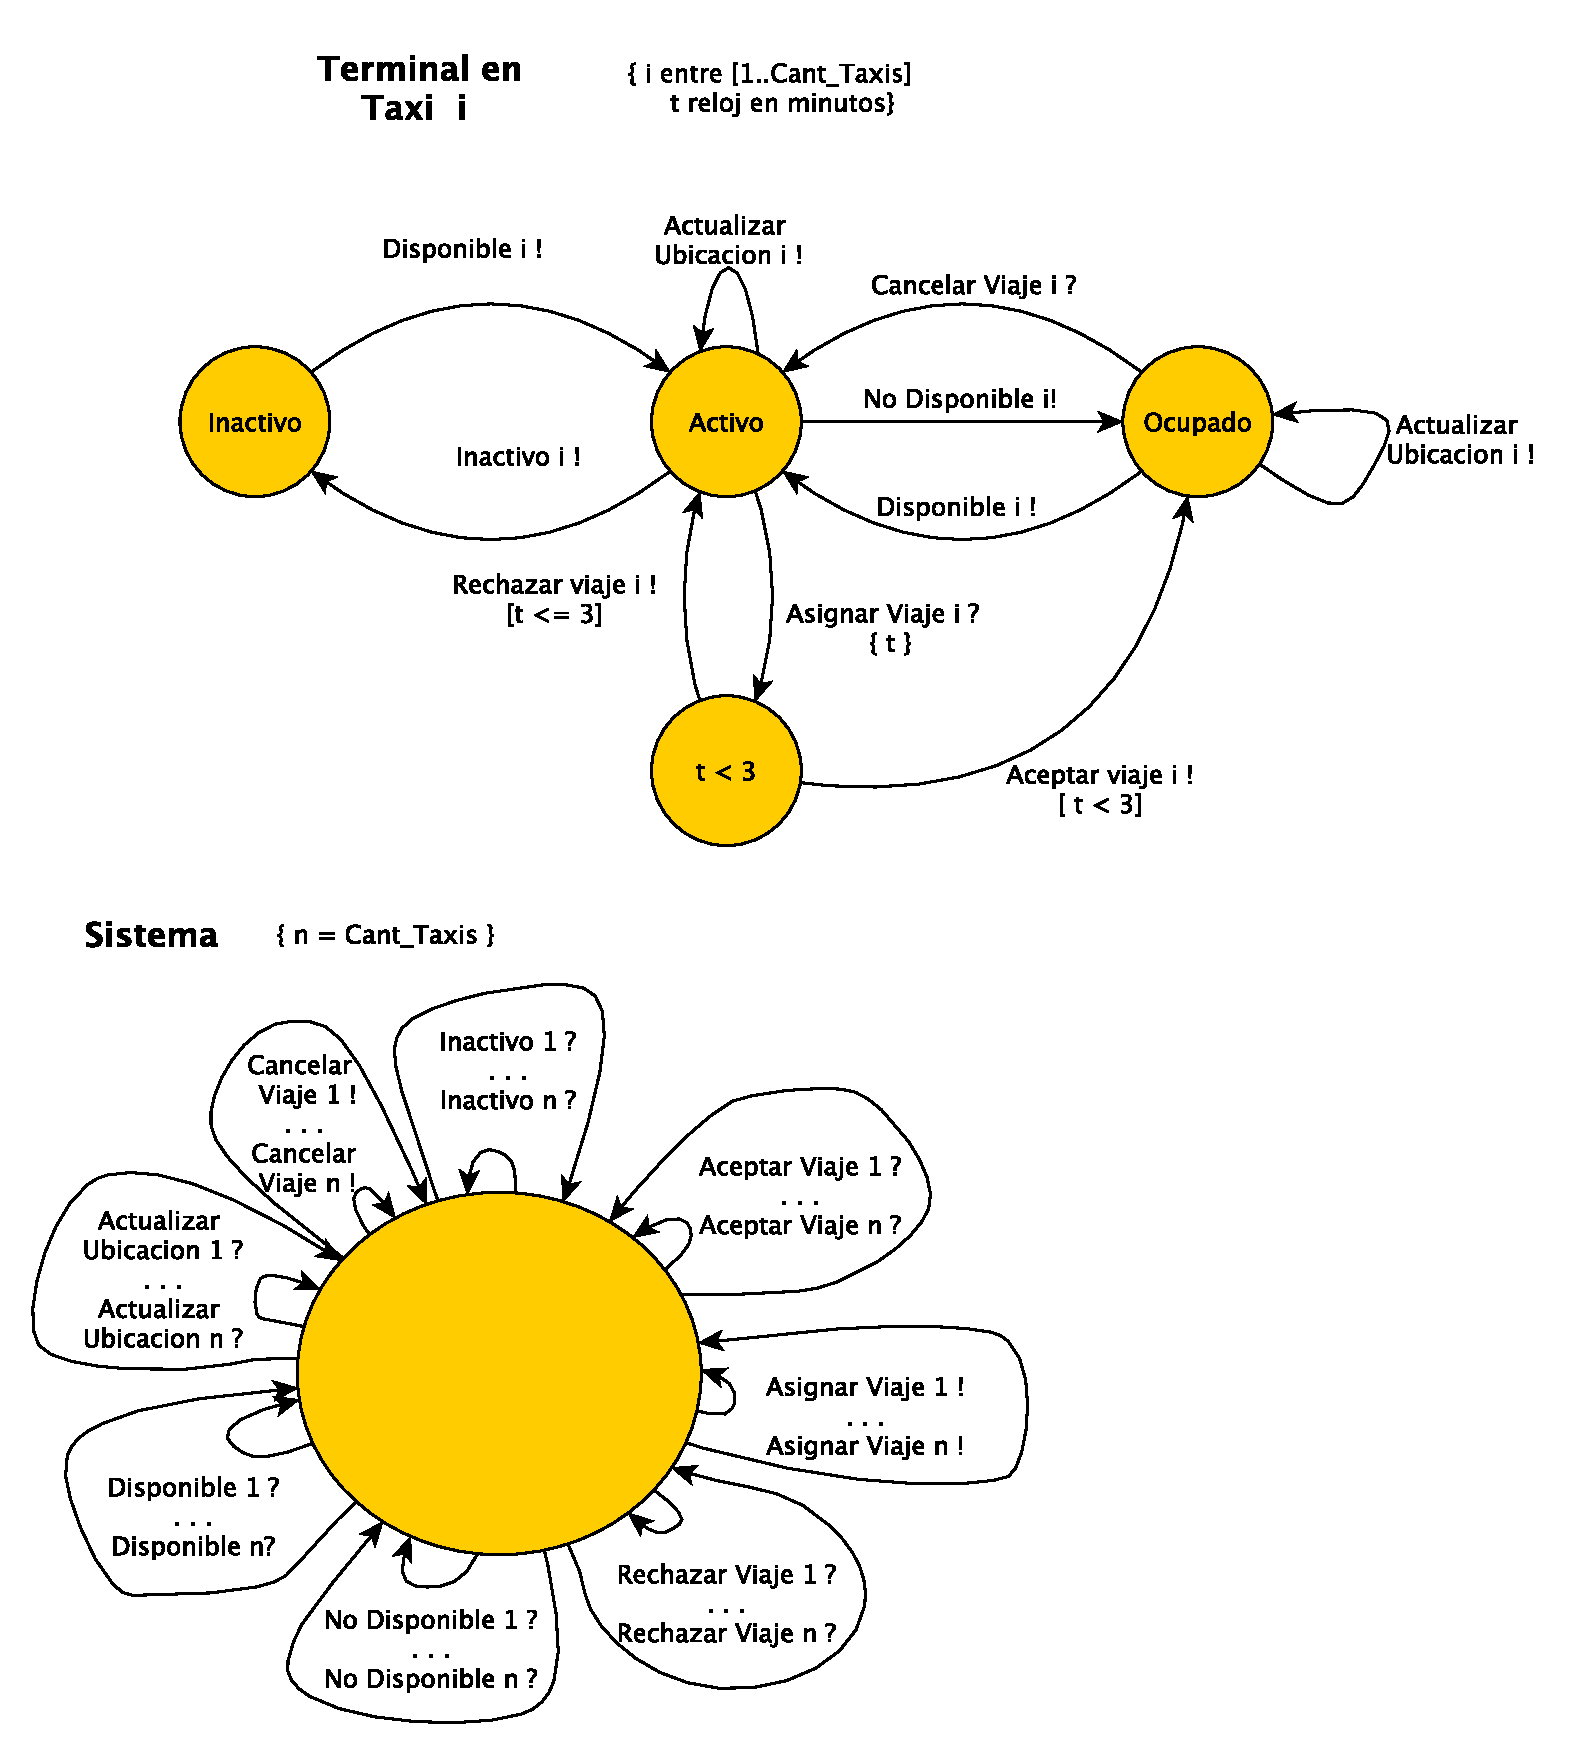
\includegraphics[scale=0.6]{diag_FSM.pdf}
\end{center}


\section{Diagramas de Actividad}

\end{document}
